\begin{center}
	\section{Estado del arte}
\end{center}

\noindent
\justify

El marco te\'orico se compone de los siguientes temas: 

\begin{itemize}
	\item M\'etodo de dispersi\'on de la matriz en fase s\'olida: m\'etodo ampliamente usado a escala de laboratorio para la extracci\'on de analitos de inter\'es de extractos procedentes de muestras biol\'ogicas. La planta de extracci\'on desarrollada fue dise\~nada con base en este m\'etodo experimental.
	\item Din\'amica de Fluidos Computacional: herramienta computacional ampliamente usada para el an\'alisis de procesos que emplean fluidos de car\'acter laminar o turbulento, gaseoso o l\'iquido y de tipo Newtoniano o no Newtoniano.
	\item M\'etodo de Elementos Discretos: m\'etodo num\'erico que permite modelar la interacci\'on din\'amica de procesos mec\'anicos que emplean part\'iculas. 
	\item M\'etodo CFD-DEM: acoplamiento entre la Din\'amica de Fluidos Computacional (CFD, por sus siglas en ingl\'es) y el M\'etodo de Elementos Discretos (DEM, por sus siglas en ingl\'es). Permite analizar problemas que emplean tanto fluidos como part\'iculas.
	\item Sedimentaci\'on: expone el fen\'omeno f\'isico base empleado para la separaci\'on de mezclas s\'olido-l\'iquido. A su vez, explica los sistemas de sedimentaci\'on conocidos en la literatura; enfoc\'andose en la metodolog\'ia de dise\~no te\'orico de sedimentadores de placas inclinadas para la propuesta de un dise\~no inicial del sistema de eluci\'on y filtrado de la planta de extracci\'on.
\end{itemize}

\begin{center}
	\section{M\'etodo MSPD}
\end{center}

\noindent
\justify

El m\'etodo de dispersi\'on de la matriz en fase s\'olida (MSPD, por sus siglas en ingl\'es) ha sido ampliamente utilizado para el estudio de muestras biol\'ogicas. Existen m\'as de 250 publicaciones en las que se emplea este m\'etodo extractivo para el an\'alisis de extractos de distintas naturalezas $^{\cite{barker2007}}$. Esto se debe a la alta eficiencia y bajo costo de este m\'etodo de extracci\'on. 

\noindent
\justify

Consiste, b\'asicamente, de tres etapas (como se puede observar en la Figura \ref{mspd}):

\begin{enumerate}
	\item Maceraci\'on de la muestra con un \textit{agente dispersante} (material particulado, normalmente compuesto de s\'ilice).
	\item Homogenizaci\'on de la muestra macerada en la columna.
	\item Eluci\'on con solvente y filtrado de la mezcla \textit{solvente - extracto}.
\end{enumerate}

\begin{figure}[h!]
\centering
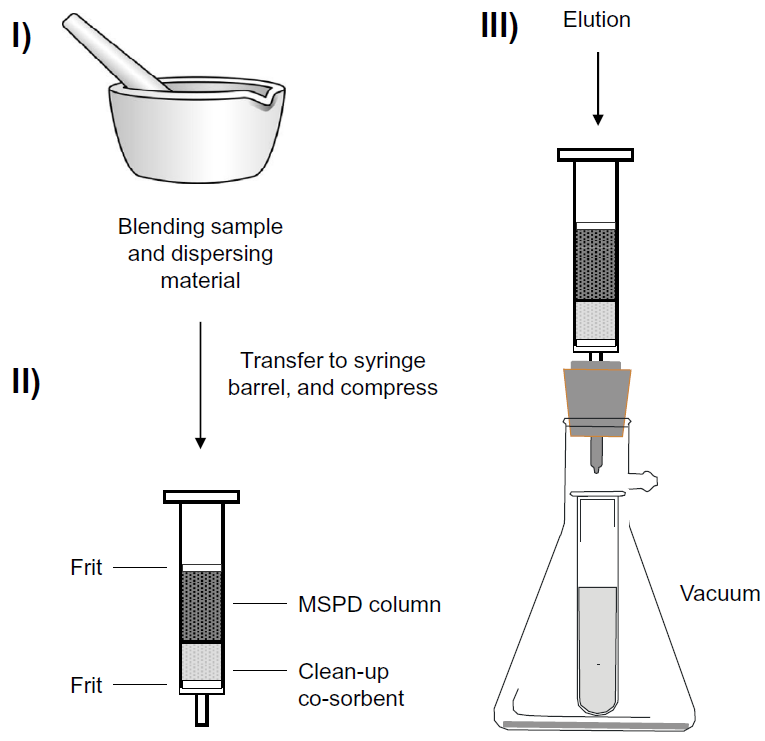
\includegraphics[width=0.8\textwidth]{Images/mspd.PNG}
\caption{M\'etodo MSPD$^{\cite{Capriotti2015}}$.}
\label{mspd}
\end{figure}

\subsection{Factores a considerar en la extracci\'on MSPD}

\noindent
\justify

Hay varios factores a considerar en la extracci\'on MSPD, que incluye:

\begin{enumerate}
	\item \textit{Efecto del tama\~no de part\'icula media:} tama\~nos de part\'icula peque\~nos (entre $3$ - $10 \, \mu m$) requiere de grandes tiempos de eluci\'on y altos gradientes de presi\'on para obtener un flujo adecuado. 
	\item \textit{Agente dispersante:} el uso de silicatos infravalorados, como la arena de r\'io, para la maceraci\'on de muestras presenta resultados diferentes a los reportados con agentes dispersantes como el $C_{18}$ o el $C_8$. A pesar de que el mismo principio de disrupci\'on de la matriz se conserva, debido a la abrasi\'on, es probable que se de una interacci\'on qu\'imica no deseada entre silicatos infravalorados y algunos de los flavonoides del extracto.
	\item \textit{Relaci\'on m\'asica:} la mejor relaci\'on m\'asica reportada en la literatura frecuenta ser una relaci\'on 1 a 4 $^{\cite{barker2007}}$, aunque puede variar de una aplicaci\'on a otra. 
	\item \textit{Solvente:} el vertimiento del solvente en la columna MSPD tiene el fin de aislar analitos espec\'ificos o familias de compuestos. El tipo de solvente, y la polaridad de este, define la composici\'on final del extracto. Existen estudios en donde se ha demostrado un incremento en el rendimiento extractivo al emplear solventes a temperaturas superiores a la temperatura ambiente e inferiores a los $60 \left[ \degree C \right]^{\cite{Vieira2019}}$. 
\end{enumerate}

\subsection{Extracci\'on en fase s\'olida}

\noindent
\justify

El m\'etodo MSPD presenta diferencias claras respecto a la extracci\'on fase s\'olida cl\'asica (SPE, por sus siglas en ingl\'es); entre ellas$^{\cite{barker2007}}$:
\begin{enumerate}
	\item Al emplear el m\'etodo MSPD, se consigue una disrupci\'on completa de la muestra en part\'iculas de reducido tama\~no, incrementando el \'area de extracci\'on. En SPE, la disrupci\'on de la muestra se considera un paso \textit{adicional}, donde muchos de los compuestos se descartan al procesar la muestra para la columna SPE. 
	\item En SPE, la muestra es usualmente absorbida en la parte superior de la columna y no a trav\'es de ella, como en el m\'etodo MSPD.
	\item La interacci\'on f\'isica y qu\'imica de los compuestos del sistema son mayores en el m\'etodo MSPD y diferentes, en diversos sentidos, de aquellos apreciados en el SPE cl\'asico, incluyendo otras formas de cromatograf\'ia l\'iquida.
\end{enumerate}

\newpage

\subsection{Prototipo a escala}

\noindent
\justify

Se han desarrollado estudios experimentales sobre un prototipo a escala de una planta de extracci\'on con capacidad productiva de $1 [kg / bache]$, tres baches al d\'ia. El flujo de trabajo se puede apreciar en la Figura \ref{cadena}.

\begin{figure}[h!]
	\centering
	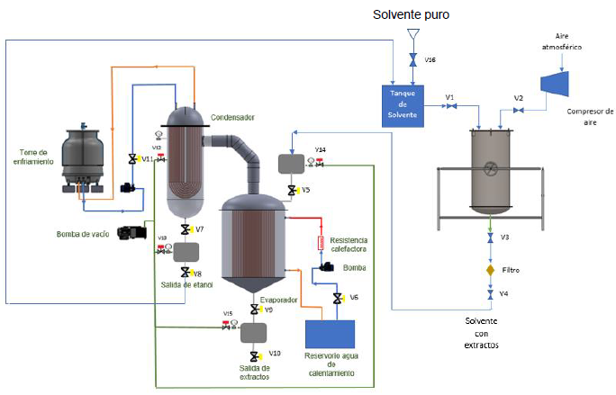
\includegraphics[width=1.1\textwidth]{Images/planta.PNG}
	\caption{Prototipo desarrollado$^{\cite{Proyecto, Patente2018}}$.}
	\label{cadena}
\end{figure}

La invenci\'on desarrollada consiste de:
\begin{itemize}
	\item Molino de bolas dise\~nado como recipiente a presi\'on.
	\item Unidad compresora de aire.
	\item Evaporador.
	\item Condensador.
	\item Sistema de calentamiento de agua por resistencia el\'ectrica.
	\item Torre de enfriamiento.
\end{itemize}




\subsection{Din\'amica de Fluidos Computacional} \label{DFC}

\noindent
\justify

La \textit{Din\'amica de Fluidos Computacional} (CFD, por sus siglas en ingl\'es) es una herramienta computacional ampliamente usada en ingenier\'ia para el desarrollo de simulaciones num\'ericas que involucren fluidos. Emplea como m\'etodo base el m\'etodo de vol\'umenes finitos (FVM). Este m\'etodo num\'erico transforma las ecuaciones diferenciales parciales, que representan las leyes conservativas, en ecuaciones algebraicas discretas sobre vol\'umenes finitos. 

\noindent
\justify

Inicia con la discretizaci\'on del dominio en elementos no superpuestos. Las ecuaciones diferenciales son discretizadas (transformadas) en ecuaciones algebraicas al integrarlas sobre cada dominio de los elementos. El sistema de ecuaciones algebraicas es luego resulto para calcular los valores de las variables dependientes de cada elemento. Algunos de los t\'etminos en la ecuaci\'on de conservaci\'on se convierten en flujos que se eval\'uan sobre las caras de los elementos. Es `sencillo' evaluar condiciones de frontera, tanto de tipo \textit{Dirichlet} como \textit{Neumann}, de manera no invasiva, dado que las variables desconocidas se eval\'uan en los centroides de los elementos, no en las caras de los mismos, como se aprecia en la Figura \ref{elemento}. Estas caracter\'istias lo hacen adecuado para que la simulaci\'on presente una variedad de aplicaciones que involucran: flujo de fluidos y transferencia de calor y masa.

\noindent
\justify

B\'asicamente, con este m\'etodo num\'erico se busca resolver los siguientes grupos de ecuaciones:

\begin{itemize}
	\item Ecuaci\'on de continuidad:
	\begin{equation*}
		\frac{\partial u}{\partial x} + \frac{\partial v}{\partial y} = 0
	\end{equation*}
	\item Ecuaciones de momento:
	\begin{equation*}
			\frac{\partial u}{\partial t} + u \frac{\partial u}{\partial x} + v \frac{\partial u}{\partial y} = - \frac{1}{\rho} \frac{\partial p}{\partial x} + \frac{\mu}{\rho} \left( \frac{\partial ^2 u}{\partial x ^2} + \frac{\partial ^2 u}{\partial y ^2} \right)
	\end{equation*}
	\begin{equation*}
			\frac{\partial v}{\partial t} + u \frac{\partial v}{\partial x} + v \frac{\partial v}{\partial y} = - \frac{1}{\rho} \frac{\partial p}{\partial y} + \frac{\mu}{\rho} \left( \frac{\partial ^2 v}{\partial x ^2} + \frac{\partial ^2 v}{\partial y ^2} \right)
	\end{equation*}
\end{itemize}

\noindent
\justify

De estas ecuaciones, los componentes desconocidos suelen ser la presi\'on y velocidad. Se requieren condiciones iniciales y de frontera para definir el problema.No hay una ecuaci\'on espec\'ifica para definir la presi\'on. Para flujos incompresibles, la presi\'on es el campo que hace que la velocidad logre cumplir la ley de la conservaci\'on de la masa$^{\cite{Abou-Hweij2020}}$.

\noindent
\justify

Los m\'etodos num\'ericos se enfocan tanto en el proceso de discretizaci\'on como en el m\'etodo de soluci\'on del grupo de ecuaciones algebraicas obtenidas. La \textbf{precisi\'on} de una soluci\'on num\'erica est\'a arraigada al m\'etodo de discretizaci\'on$^{\cite{Bao2021}}$.

\begin{figure}[h!]
	\centering
	\begin{tikzpicture}
 		\draw (0,0) rectangle (12,7);
 		\foreach \x in {1,...,4}{
			\draw (\x*3,0) -- (\x*3,7); 		
 		}
 		\foreach \y in {1,...,3}{
			\draw (0, \y*2.33) -- (12,\y*2.33); 		
 		}	
 		\draw[pattern=north west lines, pattern color=blue!55!red] (3,2.33) rectangle (6,4.66);	
 		\draw[fill=cyan] (4.5,3.5) circle (0.2cm);
 		\draw[-triangle 90, fill=black] (7.5,3.5) -- (4.7,3.5);
 		\node[align=right] at (7.5,3.5) {Centroide del \\ elemento};
 		\node[color=black] at (4.5,3) {Elemento};
 		\draw (9,4.66) circle (0.1cm);
 		\draw[-triangle 90, fill=black] (10.5,5.3) -- (9.15,4.8);
 		\node[align=right] at (10.5,5.5) {(V\'ertice)};
	\end{tikzpicture}
	\caption{Discretizaci\'on del dominio (malla cartesiana).}
	\label{elemento}
\end{figure}

\newpage

\noindent
\justify

Existen dos tipos de mallas para el an\'alisis mediante CFD, como se aprecia en la Figura \ref{mallas}.

\begin{figure}[h!]
	\centering
	\begin{subfigure}[b]{0.48\textwidth}
		\centering
		\begin{adjustbox}{max width = \textwidth}
		\begin{tikzpicture}
			\begin{axis}[grid=both,view={70}{40},colormap/viridis]
  				\addplot3+[surf,mesh/rows=11,mesh/ordering=colwise,no marks] file {malla.txt};
			\end{axis}
		\end{tikzpicture}
		\end{adjustbox}
		\caption{Malla estructurada.}
	\end{subfigure}
	\hfill
	\begin{subfigure}[b]{0.5\textwidth}
		\centering
		\begin{adjustbox}{max width = \textwidth}
		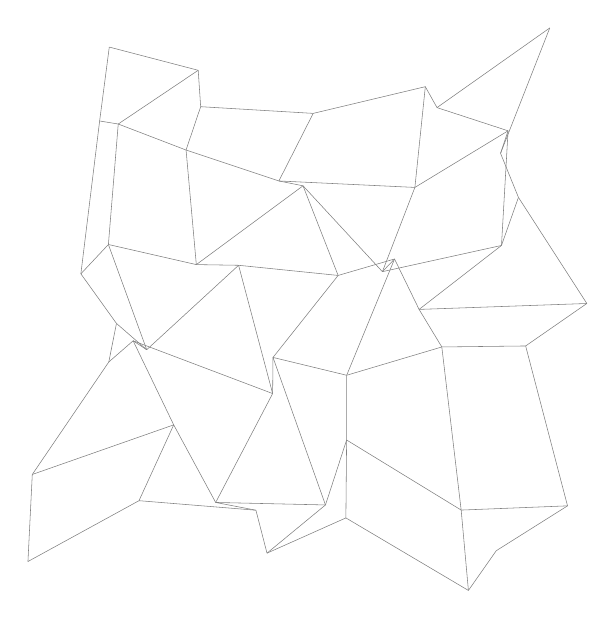
\begin{tikzpicture}
			\foreach \i [evaluate={\ii=int(\i-1);}] in {0,...,6}{
  			\foreach \j [evaluate={\jj=int(\j-1);}] in {0,...,6}{
    			\coordinate [shift={(\j,\i)}] (n-\i-\j) at (rand*270:1/2+rnd/8);
				\ifnum\i>0
  					\draw [help lines] (n-\i-\j) -- (n-\ii-\j);
				\fi
				\ifnum\j>0
  					\draw [help lines] (n-\i-\j) -- (n-\i-\jj);
				\fi
			}}
		\end{tikzpicture}
		\end{adjustbox}
	\caption{Malla no estructurada.}
	\end{subfigure}
	\caption{Tipos de mallas.}
	\label{mallas}
\end{figure}

\noindent
\justify

La conversi\'on de las ecuaciones diferenciales parciales requieren la discretizaci\'on del dominio de estudio; que, a su vez, depende de la dimensionalidad del problema.

\subsubsection{Solucionadores}

\noindent
\justify

Existen diferentes m\'etodos de soluci\'on de sistemas de ecuaciones algebraicas que pueden ser: \textit{exactos} o \textit{iterativos}. Los solucionadores que emplean m\'etodos exactos no suelen usarse en simulaciones num\'ericas debido al alto costo computacional. B\'asicamente tratan de resolver el sistema matricial $A \phi = B \rightarrow \phi = A^{-1} B$. 

\noindent
\justify

Los m\'etodos iterativos suelen basarse en la l\'ogica de \textit{suposici\'on} y \textit{corroboraci\'on}. El m\'etodo de Gauss - Seidel$^{\cite{Bai2021}}$, por ejemplo, inicia suponiendo el valor de una variable, corrobor\'andola con el c\'alculo de las dem\'as; en caso de no coincidir, su supone el resultado final de la variable supuesta, donde se vuelve a corroborar hasta que el supuesto y la corroboraci\'on coincidan o hasta que el margen de error sea tolerable.

\subsubsection{Metodolog\'ias de verificaci\'on y validaci\'on} \label{verified}

\noindent
\justify

Tienen por objetivo garantizar el menor \textit{error computacional} posible. Entre ellas se destacan:

\begin{itemize}
	\item \textit{Simple}: estudio de la evoluci\'on global o local de una variable debido al refinamiento de malla, como se aprecia en la Figura \ref{valsimple}.
	\begin{figure}[h!]
	\centering
	\begin{tikzpicture}
		\begin{axis}[
			domain = 0:1000,
			grid = both, minor tick num=2,
			title = \textbf{Validaci\'on por refinamiento de malla},
			xlabel = N\'umero de nodos,
			ylabel = Valor,
			legend pos = outer north east,
			restrict y to domain* = 0:100,
			width=10cm, height=8cm
		]
		\addplot[blue, line width=2pt] {\val};
		\addplot[
        scatter,scatter src=explicit symbolic,
        scatter/classes={
            a={mark=o,black},
            b={mark=triangle*,red},
            c={mark=o,draw=black,fill=black}
        }
    ]
    table[x=x,y=y,meta=label]{
        x	y	label
		10	30	a
		15	32	a
		30	43	a
		60	55	a
		100	70	a
		300	80	a
		600	92	a
		800	95	a
		1000	96	a

    };
		\legend{Te\'orico, Num\'erico};
		\end{axis}
	\end{tikzpicture}
	\caption{M\'etodo de validaci\'on simple.}
	\label{valsimple}
	\end{figure}
	\item \textit{Detallada}: se basa en la extrapolaci\'on generalizada de Richardson y en el \'indice de convergencia de malla (GCI).
	\item \textit{Experimentaci\'on}: se validan los resultados con estudios experimentales.
\end{itemize}

\subsubsection{An\'alisis bidimensional - 2D} \label{CFD2D}

\noindent
\justify

Para an\'alisis bidimensional, se busca resolver la Ecuaci\'on \ref{2DCFD}.

\begin{equation}
\underbrace{\rho \frac{\partial \phi}{\partial t}}_{\text{transitorio}} + \underbrace{\rho u \frac{\partial \phi}{\partial x} + \rho v \frac{\partial \phi}{\partial y}}_{\text{convectivo}} = \underbrace{ \frac{\partial}{\partial x} \left( \Gamma \frac{\partial \phi}{\partial x} \right) + \frac{\partial}{\partial y} \left( \Gamma \frac{\partial \phi}{\partial y} \right)}_{\text{difusivo}} + \underbrace{S_{\phi}}_{\text{fuente}}
\label{2DCFD}
\end{equation}

\noindent
\justify

La discretizaci\'on del dominio se realiza acorde a la Figura \ref{dis2D}.

\begin{figure}[h!]
\centering
\begin{tikzpicture}
\draw (0,0) rectangle (6,6);
\newcounter{contx} %counter
\setcounter{contx}{0}
\newcounter{conty} %counter
\setcounter{conty}{0}
\foreach \x in {0,1.5,3,4.5}
    \foreach \y in {0,1.5,3,4.5}
      {
        \draw (\x,\y) rectangle (\x + 1.5, \y + 1.5);
        \draw[fill=black] (\x + 0.75, \y + 0.75) circle (0.5mm);
        \stepcounter{conty}
        \ifnum \value{contx}<3
        	\draw[red, -triangle 90, fill=red] (\x+1.3, \y + 0.75) -- (\x+1.7, \y + 0.75);
        \fi
        \ifnum \value{conty}=4
        	\setcounter{conty}{0}
        	\stepcounter{contx}
        \else
        	\draw[blue, -triangle 90, fill=blue] (\x+0.75, \y + 1.3) -- (\x+0.75, \y + 1.7);
        \fi
      }

\foreach \x in {0,1.5,3,4.5}
	{
		\draw[fill=black] (\x + 0.75, 0) circle (0.5mm);
		\draw[fill=black] (\x + 0.75, 6) circle (0.5mm);
	}

\foreach \y in {0,1.5,3,4.5}
	{
		\draw[fill=black] (0, \y + 0.75) circle (0.5mm);
		\draw[fill=black] (6, \y + 0.75) circle (0.5mm);
	}

\node at (2.5,2.5) {P};
\node at (4,2.5) {E};
\node at (2.5,4) {N};
\node at (2.5,1) {S};
\node at (1,2.5) {W};

\end{tikzpicture}
\caption{Discretizaci\'on dominio bidimensional.}
\label{dis2D}
\end{figure}

\noindent
\justify

Existen diferentes enfoques para el an\'alisis de problemas bidimensionales, entre ellos se encuentran: diferencias centradas, \textit{upwind} e h\'ibrido. El acercamiento por diferencias centradas asume una variaci\'on lineal de $\phi$ entre nodos para una malla uniforme, de modo que:

\begin{equation}
\begin{array}{c}
	a_P \phi _P = a_E \phi _E  + a_W \phi _W + a_N \phi _N + a_S \phi _S + b \\
	a_E = D_e - F_e/2 \\
	a_W = D_w + F_w/2 \\
	a_N = D_n - F_n/2 \\
	a_S = D_s + F_s/2 \\
	a_P = a_E + a_W + a_N + a_S + \rho \frac{\Delta x \Delta y}{\Delta t} + \left(F_e - F_w + F_n - F_s \right) \\
	b = \rho \frac{\Delta x \Delta y}{\Delta t} \phi _P ^0 + S \Delta x \Delta y
\end{array}
\end{equation}

\subsection{M\'etodo de Elementos Discretos}


\noindent
\justify

El m\'etodo de elementos discretos (DEM) es un m\'etodo que modela fuerzas interpart\'icula basadas en par\'ametros de elasticidad y la superposici\'on de part\'iculas no deformadas, que se entiende como la cantidad de deformaci\'on necesaria para que puedan, f\'isicamente, ocupar el espacio en su actual configuraci\'on. Requiere de seis grados de libertad en cuerpos r\'igidos: tres en dos dimensiones y seis en tres dimensiones.

\begin{figure}[h!]
	\centering
	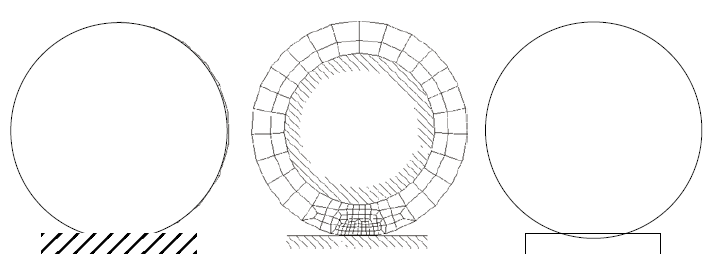
\includegraphics[width=\textwidth]{Images/DEM.PNG}
	\label{dem}
	\caption{Comparaci\'on entre metodolog\'ias de an\'alisis de part\'iculas para una esfera suave deformada en un plano: situaci\'on f\'isica real (izquierda), modelo analizado con el m\'etodo de elementos finitos (centro) y modelo con el m\'etodo de elementos discretos (derecha). Fuente: \v Smilauer 2015$^{\cite{Smilauer2015}}$.}
\end{figure}

\noindent
\justify

El principio de este m\'etodo es el de computar las fuerzas proporcionales a la superposici\'on geom\'etrica de las part\'iculas empleadas. Para part\'iculas esf\'ericas, o circulares, las fuerzas involucradas son de tipo central; a diferencia de otras configuraciones geom\'etricas, debido a que deben caracterizar las fuerzas en la forma `d\'ebil' y `fuerte'. 

\noindent
\justify

Una simulaci\'on que emplea este m\'etodo num\'erico, normalmente se rige bajo los siguientes pasos:

\begin{enumerate}
	\item Detecci\'on de colisi\'on entre part\'iculas.
	\item Creaci\'on de una nueva interacci\'on y determinaci\'on de diferentes propiedades, entre ellas la rigidez.
\end{enumerate}

\noindent
\justify

Para interacciones ya existentes:

\begin{enumerate}
	\item Evaluaci\'on de deformaci\'on.
	\item Computaci\'on del esfuerzo basada en la deformaci\'on.
	\item Aplicaci\'on de fuerzas en la interacci\'on entre part\'iculas.
\end{enumerate}

\subsubsection{Detecci\'on de una colici\'on} \label{detect}

\noindent
\justify

La detecci\'on \textit{exacta} de colisi\'on entre dos part\'iculas requiere de un alto costo computacional. Tomando una pareja de cuerpos $i$ y $j$ y su colisici\'on `exacta' (en el sentido de precisi\'on admisible por la implementaci\'on num\'erica) presentadas en los puntos $P_i$ y $P_j$ la detecci\'on procede en los siguientes dos puntos:

\begin{enumerate}
	\item Detecci\'on de colisi\'on r\'apida usando puntos aproximados $\widetilde{P}_i$ y $\widetilde{P}_j$; siendo estos preconstrucciones en el modo que caracter\'isticas individuales $P_i$ y $P_j$ satisfacen la siguiente condici\'on mostrada en la Ecuaci\'on \ref{cond}.
	\begin{equation}
		\forall x \in R^3 : x \in P_i \rightarrow x \in \widetilde{P}_i
		\label{cond}
	\end{equation}
	De igual manera para $P_j$. El predicado aproximaado se conoce como `volumen l\'imite', siguiendo lo siguiente:
	\begin{equation}
		\left(\widetilde{P}_i \cap \widetilde{P}_j \right) = {\O} \rightarrow \left( P_i \cap P_j \right) = {\O}
		\label{imposible}
	\end{equation}
	\item Al filtrar las colisiones imposibles mediante la Ecuaci\'on \ref{imposible}, algoritmos de detecci\'on de mayor costo computacional pueden ser impementados al filtrar falsas parejas de colisi\'on restantes, como se observa en la Figura \ref{colision}.
	\begin{equation}
		\left(\widetilde{P}_i \cap \widetilde{P}_j \right) \neq {\O} \wedge \left(P_i \cap P_j \right) = {\O}
	\end{equation}
\end{enumerate}

\begin{figure}[h!]
\centering
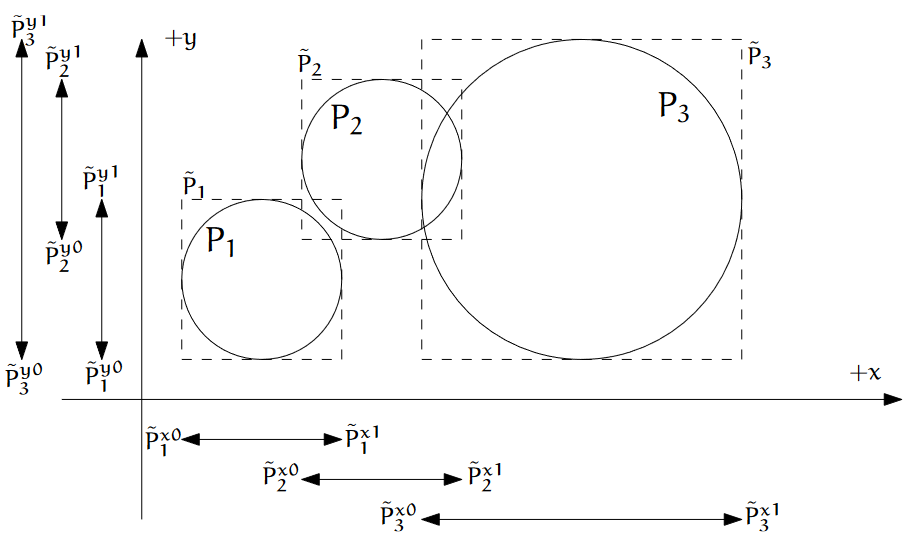
\includegraphics[width=0.9\textwidth]{Images/Colision.PNG}
\caption{Detecci\'on de colisi\'on entre part\'iculas. Fuente: \v Smilauer 2015$^{\cite{Smilauer2015}}$.}
\label{colision}
\end{figure}

\noindent
\justify

Yade$^{\cite{Smilauer2015}}$ emplea un algoritmo conocido como ``\texttt{Aabb}" (\textit{Caja de contorno para alineaci\'on de eje}, por sus siglas en ingl\'es); visualmente, consisten en los rect\'angulos de contorno que rodean cada esfera de la Figura \ref{colision}. Cada caja de contorno es usada como $\widetilde{P}_i$; estando definida cada una por sus esquinas $\varepsilon R^3$ siendo $\widetilde{P}_i ^{x0}$ y $\widetilde{P}_i ^{x1}$ las coordenadas en el eje $x$ de la esfera $P_1$, por ejemplo. 

\noindent
\justify

La presencia de superposici\'on entre part\'iculas entre dos \texttt{Aabb}'s se determina mediante el conjunto de superposici\'on separada de intervalos sobre cada eje. Est\'a representada por la Ecuaci\'on \ref{overlap:dem}.

\begin{equation}
	\left(\widetilde{P}_i \cap \widetilde{P}_j \right) \neq {\O} \Longleftrightarrow \bigwedge_{w \epsilon \{x,y,z \}} \left[\left(\left(\widetilde{P}_i ^{w0}, \widetilde{P}_i ^{w1} \right) \cap \left(\widetilde{P}_j ^{w0}, \widetilde{P}_j ^{w1} \right) \right) \neq {\O} \right] 
	\label{overlap:dem}
\end{equation}

\begin{center}
	\section{M\'etodo CFD-DEM}
\end{center}

\noindent
\justify

En el acoplamiento cl\'asico entre CFD-DEM, el flujo se resuelve a trav\'e del m\'etodo CFD basado en malla, mientras que la fase s\'olida es modelada mediante DEM para cada part\'icula sujeta a trav\'es de fuerzas hidrodin\'amicas, fuerzas de cuerpo (como la gravedad) y a trav\'es de fuerzas de contacto, actualizando valores de velocidad y posici\'on conforme a la segunda ley de Newton (Hoomans \textit{et al.}, 1996; Tsuji \textit{et al.}, 1993; Xu y Yu, 1997). En principio, todos los m\'etodos CFD pueden acoplarse con DEM; lo que ha dado origen a diferentes m\'etodos discretos y continuos, tal como el m\'etodo de Lattice Boltzmann (LBM), Hidrodin\'amica de Part\'iculas Suaves (SPH), m\'etodos de Diferencias Finitas y Vol\'umenes Finitos (FVM).

\noindent
\justify

Gran parte de las simulaciones reportadas en la literatura comprenden modelos 2D o sistemas prototipados de peque\~na escala. En busca de acelerar los tiempos de simulaci\'on e incrementar la eficiencia computacional, se han desarrollado t\'ecnicas de computaci\'on paralela; donde gran parte de los esfuerzos han sido enfocados en la paralelizaci\'on del DEM. Muchos algoritmos se han propuesto para lograr este hecho, como la t\'ecnica de espejo de dominio (Damana, \textit{et al.}, 2006; Washington y Meegoda, 2003), el m\'etodo de subconjunto de part\'iculas (Kafui \textit{et al.}, 2011) y m\'etodos de descomposici\'on de dominios (Amritkar \textit{et al.}, 2014; Tsuji \textit{et al.}, 2008). El uso de estos algoritmos depende de la arquitectura del hardware. La paralelizaci\'on sobre memoria compartida del sistema se alcanza, normalmente, empleando \textit{OpenMP} (``Open Multi-Processing", por sus siglas en ingl\'es), mientras que el MPI (Interfaz de Paso de Mensajes) se emplea en sistemas de memoria distirbuida (Rabenseifner \textit{et al.}, 2009). Por ejemplo, Tsuji \textit{et al.} (2008) paralelizaron una simulaci\'on en CFD-DEM usando MPI para el intercambio de informaci\'on entre 16 CPUs, reportando el comportamiento fluidodin\'amico de 4.5 millones de part\'iculas en un medio gaseoso; empleando el m\'etodo unidimensional de descomposici\'on de dominio.

\subsection{Fase del solvente}

\noindent
\justify

En un modelo CFD-DEM, la fase del fluido se resuleve en el nivel computacional en cada elemento de la malla (ver Figura \ref{elemento}) empleando un marco de referencia Euleriano mientras que el movimiento de la part\'icula se sigue a trav\'es de un marco de referencia Lagrangiano. Para lograr el acoplamiento de fase, es necesario interpolar las propiedades de las part\'iculas a los centroides de los elementod CFD y las propiedades del fluido a la posici\'on de cada part\'icula. Como se muestra en la Figura \ref{particle}, se crean dos mallas alineadas de b\'usqueda: la malla de b\'usqueda de part\'iculas (amarilla) y la malla de b\'usqueda de fluido (azul). 

\begin{figure}[h!]
	\centering
	\begin{subfigure}[b]{0.3\textwidth}
		\centering
		\begin{adjustbox}{max width = \textwidth}
		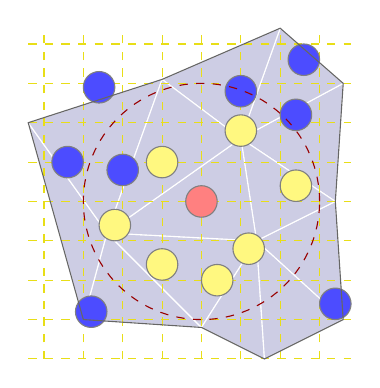
\begin{tikzpicture}
		%---Interno---
	%1 - (-1.2, -0.4)
	\draw[white, fill=blue!30!gray!30!white] (-1.5, -1.5) -- (0,-1.6) -- (-1.2, -0.4) -- cycle;
	\draw[white, fill=blue!30!gray!30!white] (-2.2, 1) -- (-1.5,-1.5) -- (-1.2, -0.4) -- cycle;
	\draw[white, fill=blue!30!gray!30!white] (-2.2, 1) -- (-0.5, 1.55) -- (-1.2, -0.4) -- cycle;
	%2 - (0.7, -0.5)
	\draw[white, fill=blue!30!gray!30!white] (-1.2, -0.4) -- (0,-1.6) -- (0.7, -0.5) -- cycle;
	\draw[white, fill=blue!30!gray!30!white] (0.8,-2) -- (0,-1.6) -- (0.7, -0.5) -- cycle;
	\draw[white, fill=blue!30!gray!30!white] (1.8,-1.5) -- (0.8,-2) -- (0.7, -0.5) -- cycle;
	\draw[white, fill=blue!30!gray!30!white] (1.8,-1.5) -- (1.7,0) -- (0.7, -0.5) -- cycle;
	%3 - (0.5,0.8)
	\draw[white, fill=blue!30!gray!30!white] (1.7,0) -- (1.8,1.5) -- (0.5, 0.8) -- cycle;
	\draw[white, fill=blue!30!gray!30!white] (1.7,0) -- (0.7, -0.5) -- (0.5, 0.8) -- cycle;
	\draw[white, fill=blue!30!gray!30!white] (1,2.2) -- (1.8,1.5) -- (0.5, 0.8) -- cycle;
	\draw[white, fill=blue!30!gray!30!white] (-0.5,1.55) -- (1,2.2) -- (0.5, 0.8) -- cycle;
	\draw[white, fill=blue!30!gray!30!white] (-1.2,-0.4) -- (0.7,-0.5) -- (0.5, 0.8) -- cycle;
	\draw[white, fill=blue!30!gray!30!white] (-1.2,-0.4) -- (-0.5,1.55) -- (0.5, 0.8) -- cycle;
	
	%malla
	\draw[step=0.5, dashed, yellow!90!black] (-2.2, -2) grid (1.9,2.2);
	
	%Partículas
	\draw[black!50, fill=red!50] (0,0) circle (2mm);
	\draw[black!50, fill=yellow!50] (0.6,-0.6) circle (2mm);
	\draw[black!50, fill=yellow!50] (-1.1,-0.3) circle (2mm);
	\draw[black!50, fill=yellow!50] (0.5,0.9) circle (2mm);
	\draw[black!50, fill=yellow!50] (-0.5,0.5) circle (2mm);
	\draw[black!50, fill=yellow!50] (1.2,0.2) circle (2mm);
	\draw[black!50, fill=yellow!50] (-0.5,-0.8) circle (2mm);
	\draw[black!50, fill=yellow!50] (0.2,-1) circle (2mm);
	
	\draw[black!50, fill=blue!70] (1.7,-1.3) circle (2mm);
	\draw[black!50, fill=blue!70] (-1.4,-1.4) circle (2mm);
	\draw[black!50, fill=blue!70] (-1,0.4) circle (2mm);
	\draw[black!50, fill=blue!70] (-1.7, 0.5) circle (2mm);
	\draw[black!50, fill=blue!70] (-1.3,1.45) circle (2mm);
	\draw[black!50, fill=blue!70] (1.2, 1.1) circle (2mm);
	\draw[black!50, fill=blue!70] (0.5,1.4) circle (2mm);
	\draw[black!50, fill=blue!70] (1.3,1.8) circle (2mm);
	
	%Carcasa
	\draw[black!60] (-2.2, 1) -- (-0.5, 1.55) -- (1, 2.2) -- (1.8, 1.5) -- (1.7, 0) -- (1.8, -1.5) -- (0.8, -2) -- (0, -1.6) -- (-1.5, -1.5) -- cycle;
	 
	 %Círculo rojo
	\draw[red!60!black, dashed] (0,0) circle (1.5 cm);
		\end{tikzpicture}
		\end{adjustbox}
		\caption{B\'usqueda de part\'iculas vecinas y c\'alculo de la fracci\'on de vac\'io de una part\'icula dada.}
	\end{subfigure}
	\hfill
	\begin{subfigure}[b]{0.3\textwidth}
		\centering
		\begin{adjustbox}{max width = \textwidth}
		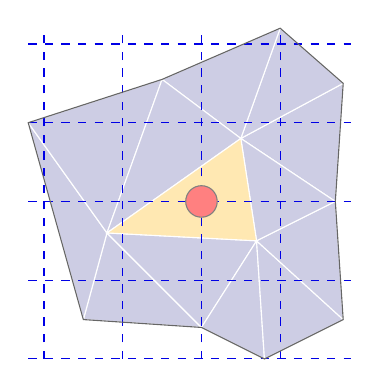
\begin{tikzpicture}
		%---Interno---
	%1 - (-1.2, -0.4)
	\draw[white, fill=blue!30!gray!30!white] (-1.5, -1.5) -- (0,-1.6) -- (-1.2, -0.4) -- cycle;
	\draw[white, fill=blue!30!gray!30!white] (-2.2, 1) -- (-1.5,-1.5) -- (-1.2, -0.4) -- cycle;
	\draw[white, fill=blue!30!gray!30!white] (-2.2, 1) -- (-0.5, 1.55) -- (-1.2, -0.4) -- cycle;
	%2 - (0.7, -0.5)
	\draw[white, fill=blue!30!gray!30!white] (-1.2, -0.4) -- (0,-1.6) -- (0.7, -0.5) -- cycle;
	\draw[white, fill=blue!30!gray!30!white] (0.8,-2) -- (0,-1.6) -- (0.7, -0.5) -- cycle;
	\draw[white, fill=blue!30!gray!30!white] (1.8,-1.5) -- (0.8,-2) -- (0.7, -0.5) -- cycle;
	\draw[white, fill=blue!30!gray!30!white] (1.8,-1.5) -- (1.7,0) -- (0.7, -0.5) -- cycle;
	%3 - (0.5,0.8)
	\draw[white, fill=blue!30!gray!30!white] (1.7,0) -- (1.8,1.5) -- (0.5, 0.8) -- cycle;
	\draw[white, fill=blue!30!gray!30!white] (1.7,0) -- (0.7, -0.5) -- (0.5, 0.8) -- cycle;
	\draw[white, fill=blue!30!gray!30!white] (1,2.2) -- (1.8,1.5) -- (0.5, 0.8) -- cycle;
	\draw[white, fill=blue!30!gray!30!white] (-0.5,1.55) -- (1,2.2) -- (0.5, 0.8) -- cycle;
	\draw[white, fill=blue!30!gray!30!white] (-1.2,-0.4) -- (-0.5,1.55) -- (0.5, 0.8) -- cycle;
	\draw[white, fill=red!30!yellow!30!white] (-1.2,-0.4) -- (0.7,-0.5) -- (0.5, 0.8) -- cycle;
	
	%malla
	\draw[step=1, dashed, blue!90!black] (-2.2, -2) grid (1.9,2.2);
	
	%Partículas
	\draw[black!50, fill=red!50] (0,0) circle (2mm);
	
	%Carcasa
	\draw[black!60] (-2.2, 1) -- (-0.5, 1.55) -- (1, 2.2) -- (1.8, 1.5) -- (1.7, 0) -- (1.8, -1.5) -- (0.8, -2) -- (0, -1.6) -- (-1.5, -1.5) -- cycle;
	 
		\end{tikzpicture}
		\end{adjustbox}
	\caption{Mapeo de una part\'icula dada dentro del fluido para interpolar sus propiedades en ese punto.}
	\end{subfigure}
	\hfill
	\begin{subfigure}[b]{0.3\textwidth}
		\centering
		\begin{adjustbox}{max width = \textwidth}
		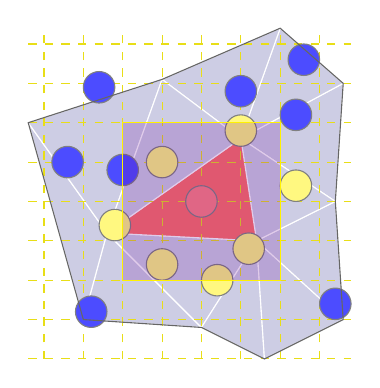
\begin{tikzpicture}
		%---Interno---
	%1 - (-1.2, -0.4)
	\draw[white, fill=blue!30!gray!30!white] (-1.5, -1.5) -- (0,-1.6) -- (-1.2, -0.4) -- cycle;
	\draw[white, fill=blue!30!gray!30!white] (-2.2, 1) -- (-1.5,-1.5) -- (-1.2, -0.4) -- cycle;
	\draw[white, fill=blue!30!gray!30!white] (-2.2, 1) -- (-0.5, 1.55) -- (-1.2, -0.4) -- cycle;
	%2 - (0.7, -0.5)
	\draw[white, fill=blue!30!gray!30!white] (-1.2, -0.4) -- (0,-1.6) -- (0.7, -0.5) -- cycle;
	\draw[white, fill=blue!30!gray!30!white] (0.8,-2) -- (0,-1.6) -- (0.7, -0.5) -- cycle;
	\draw[white, fill=blue!30!gray!30!white] (1.8,-1.5) -- (0.8,-2) -- (0.7, -0.5) -- cycle;
	\draw[white, fill=blue!30!gray!30!white] (1.8,-1.5) -- (1.7,0) -- (0.7, -0.5) -- cycle;
	%3 - (0.5,0.8)
	\draw[white, fill=blue!30!gray!30!white] (1.7,0) -- (1.8,1.5) -- (0.5, 0.8) -- cycle;
	\draw[white, fill=blue!30!gray!30!white] (1.7,0) -- (0.7, -0.5) -- (0.5, 0.8) -- cycle;
	\draw[white, fill=blue!30!gray!30!white] (1,2.2) -- (1.8,1.5) -- (0.5, 0.8) -- cycle;
	\draw[white, fill=blue!30!gray!30!white] (-0.5,1.55) -- (1,2.2) -- (0.5, 0.8) -- cycle;
	\draw[white, fill=red!95!yellow!60!white] (-1.2,-0.4) -- (0.7,-0.5) -- (0.5, 0.8) -- cycle;
	\draw[white, fill=blue!30!gray!30!white] (-1.2,-0.4) -- (-0.5,1.55) -- (0.5, 0.8) -- cycle;
	
	%malla
	\draw[step=0.5, dashed, yellow!90!black] (-2.2, -2) grid (1.9,2.2);
	
	%Partículas
	\draw[black!50, fill=red!50] (0,0) circle (2mm);
	\draw[black!50, fill=yellow!50] (0.6,-0.6) circle (2mm);
	\draw[black!50, fill=yellow!50] (-1.1,-0.3) circle (2mm);
	\draw[black!50, fill=yellow!50] (0.5,0.9) circle (2mm);
	\draw[black!50, fill=yellow!50] (-0.5,0.5) circle (2mm);
	\draw[black!50, fill=yellow!50] (1.2,0.2) circle (2mm);
	\draw[black!50, fill=yellow!50] (-0.5,-0.8) circle (2mm);
	\draw[black!50, fill=yellow!50] (0.2,-1) circle (2mm);
	
	\draw[black!50, fill=blue!70] (1.7,-1.3) circle (2mm);
	\draw[black!50, fill=blue!70] (-1.4,-1.4) circle (2mm);
	\draw[black!50, fill=blue!70] (-1,0.4) circle (2mm);
	\draw[black!50, fill=blue!70] (-1.7, 0.5) circle (2mm);
	\draw[black!50, fill=blue!70] (-1.3,1.45) circle (2mm);
	\draw[black!50, fill=blue!70] (1.2, 1.1) circle (2mm);
	\draw[black!50, fill=blue!70] (0.5,1.4) circle (2mm);
	\draw[black!50, fill=blue!70] (1.3,1.8) circle (2mm);
	
	%Carcasa
	\draw[black!60] (-2.2, 1) -- (-0.5, 1.55) -- (1, 2.2) -- (1.8, 1.5) -- (1.7, 0) -- (1.8, -1.5) -- (0.8, -2) -- (0, -1.6) -- (-1.5, -1.5) -- cycle;
	
	\draw[yellow, fill=red!40!blue, fill opacity=0.2] (-1,-1) rectangle (1,1);
		\end{tikzpicture}
		\end{adjustbox}
	\caption{Mapeo del elemento de malla CFD para el c\'alculo de t\'erminos fuente en el elemento de inter\'es.}
	\end{subfigure}
	\caption{Esquema de la aproximaci\'on por malla dual para la b\'usqueda de part\'iculas vecinas en un fluido.}
	\label{particle}
\end{figure}

\noindent
\justify

Los pasos clave con los que se basan las mallas de b\'usqueda son: detecci\'on de colisi\'on de part\'iculas (descrito en la secci\'on \ref{detect}), geometr\'ia de los elementos de malla CFD (detallado en la secci\'on \ref{CFD2D}) y el c\'alculo de fuerzas de fluido, entre otras.

\noindent
\justify

Para el c\'alculo de las fuerzas ejercidas por el fluido, se requiere conocer las propiedades del fluido en la posici\'on de la part\'icula; incluyendo el gradiente de presi\'on, la velocidad del flujo y el gradiente de velocidades (para fluidos gaseosos). Normalmente, las propiedades del fluido se `almacenan' en el centroide de los elementos de malla durante c\'alculos mediante FVM, como se muestra en la Ecuaci\'on \ref{properties}.

\begin{equation}
\phi _p = \phi _{el} + \nabla \phi _{el} \cdot r_{pc}
\label{properties}
\end{equation}

\noindent
\justify

D\'onde: $\phi _p$ y $\phi _{el}$ son las propiedades del fluido en la posici\'on de la part\'icula y el centroide del elemento, respectivamente; y $r_{pc}$ es el vector distancia que va desde el centro del elemento hasta la posici\'on de la part\'icula. 

\begin{center}
	\section{Sedimentaci\'on}
\end{center}

\noindent
\justify

La sedimentaci\'on es uno de los procesos m\'as antiguos en el tratamiento del agua y consiste en la deposici\'on de materiales s\'olidos de mayor peso que el agua.

\noindent
\justify

Existen cinco tipos de sedimentaci\'on que se clasifican de acuerdo a  la clase de part\'icuas, caracter\'isticas superficiales y concentraci\'on de las mismas:

\begin{itemize}
	\item Sedimentaci\'on \textit{discreta:} las part\'iculas no tienden a aglomerarse, mantienen su tama\~no e individualidad. Son generalmente de textura arenosa.
	\item Sedimen \textit{floculenta}: las part\'iculas floculan y tienden a agruparse durante el proceso.
	\item Sedimentaci\'on \textit{m\'asica}: la concentraci\'on de part\'iculas es tan grande que colisionan entre s\'i, sedimentando como una masa.
	\item Sedimentaci\'on por \textit{compresi\'on}: la concentraci\'on de part\'iculas es tan grande que cada una reposa sobre la otra, present\'andose una especie de soporte entre cada una de ellas; el peso de las part\'iculas superiores tiende a compactar a las inferiores.
	\item Sedimentaci\'on de \textit{alta tasa}: es una variaci\'on de la sedimentaci\'on discreta, en la que se insertan placas paralelas con el fin de aumentar la eficiencia de remoci\'on de part\'iculas.
\end{itemize}

\noindent
\justify

La \textit{sedimentaci\'on} realiza la separaci\'on de los s\'olidos m\'as densos que el agua y la \textit{filtraci\'on} separa aquellos que tienen una densidad muy cercana a la del fluido.

\subsection{Sedimentaci\'on con coagulantes}

\noindent
\justify

Se efect\'ua la decantaci\'on de part\'iculas en las c\'amaras de floculaci\'on; el tama\~no y densidad de las part\'iculas y viscosidad del agua desempae\~nar\'an un papel importante en el dimensionamiento de los sedimentadores. Las unidades podr\'an ser circulares o de flujo radial, cuadradas y rectangulares. Si los tanques sedimentadores se dise\~nan en dos o m\'as pisos, podr\'an ser de flujos independientes o de flujo \textit{zig-zag}, de manera que el flujo recorra todos los pisos de la unidad.

\subsection{Sedimentadores de \textit{placas paralelas}}

\noindent
\justify

Se trata de un tipo de sedimentador desarrollado por Hazen A, en 1904, quien expuso el siguiente principio: ``como la acci\'on de un tanque sedimentador depende de su \'area, y no de su profundidad, una subdivisi\'on horizontal producir\'ia una superficie doble para reunir sedimentos en lugar de una sencilla y duplicar\'ia la cantidad de trabajo". 

\noindent
\justify

La diferencia de los sedimentadores de tasa normal y los de alta tasa son:

\begin{itemize}
	\item El fondo del decantador no es horizontal sino inclinado.
	\item La profundidad del decantador es baja, de forma que hay que construir un n\'umero considerable de celdas superpuestas para poder tratar los vol\'umenes de agua.
	\item El flujo \textbf{debe ser laminar}, con n\'umero de Reynolds entre $80$ y $250$.
\end{itemize}

\begin{figure}[h!]
	\centering
	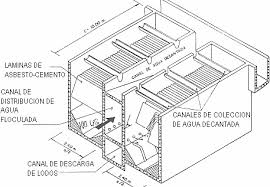
\includegraphics[width=0.7\textwidth]{Images/Sedimentacion/placas.jpg}
	\caption{Sedimentador de placas paralelas.}
	\label{placas}
\end{figure}

\noindent
\justify

Las placas presentan una inclinaci\'on, donde el agua ascendente deposita sobre ellas el material que trae en suspensi\'on. Los lodos resbalan pendiente abajo, y pueden ser recolectados en una tolva en la parte inferior de la estructura.

\begin{equation}
	V_s = \frac{V_0 S}{\sin \theta + \frac{L}{e} \cos \theta}
	\label{CargaSuperficial}
\end{equation}

\noindent
\justify

La Ecuaci\'on \ref{CargaSuperficial}, para un determinado posicionamiento de las placas, permite determinar la velocidad requerida para conseguir una velocidad cr\'itica. Es crucial mantener el n\'umero de Reynolds bajo para evitar que la turbulencia levante los lodos de la cara de las placas donde se est\'a sedimentando.

\subsection{Turbiedad}

\noindent
\justify

La turbidez es la expresi\'on de la propiedad \'optica de la muestra que causa que los rayos de la luz sean dispersados y absorbidos en lugar de ser transmitidos en l\'inea recta a trav\'es de la muestra.

\noindent
\justify

La turbiedad en el agua puede ser causada por la presencia de part\'iculas suspendidas y disueltas de gases, l\'iquidos y s\'olidos tanto org\'anicos como inorg\'anicos.

\noindent
\justify

La eliminaci\'on de la turbiedad se lleva a cabo mediante procesos de coagulaci\'on, asentamiento y filtraci\'on.

